\chapter{КОНСТРУКТОРСКИЙ РАЗДЕЛ}

\section{Проектирование архитектуры системы}

\justifying

Проектирование системы семантического поиска выполнено с использованием методологии структурного анализа IDEF0, что позволяет наглядно представить функциональную декомпозицию системы и взаимосвязи между компонентами.

\subsection{Контекстная диаграмма системы}

На рисунке \ref{idef0} представлена контекстная диаграмма IDEF0 верхнего уровня, показывающая систему семантического поиска как единый функциональный блок.

\begin{figure}[H]
	\centering
	
\includegraphics[width=0.9\textwidth]{images/IDEF0.png}
	\caption{Контекстная диаграмма IDEF0 системы семантического поиска}
	\label{idef0}
\end{figure}

Основная функция системы "Выполнить семантический поиск по документам" преобразует входные данные (корпус документов и поисковые запросы) в результаты поиска с учетом семантической близости. 

Входными данными являются:
\begin{itemize}
	\item Корпус документов в форматах PDF, DOCX, DOC
	\item Поисковые запросы пользователей
	\item Параметры обучения и поиска
\end{itemize}

Выходными данными являются:
\begin{itemize}
	\item Ранжированный список релевантных документов
	\item Обученная модель Doc2Vec
	\item Автоматические выжимки документов
	\item Статистика и метрики качества
\end{itemize}

Управляющими воздействиями выступают:
\begin{itemize}
	\item Требования к качеству поиска
	\item Ограничения по производительности
	\item Настройки пользователя
\end{itemize}

Механизмами реализации являются:
\begin{itemize}
	\item Алгоритм Doc2Vec
	\item Библиотеки обработки текстов (SpaCy, Gensim)
	\item Вычислительные ресурсы системы
\end{itemize}

\subsection{Декомпозиция основных процессов}

Детальная декомпозиция системы представлена на диаграмме IDEF0 первого уровня (рисунок \ref{idef1}), где выделены три основных процесса.

\begin{figure}[H]
	\centering
	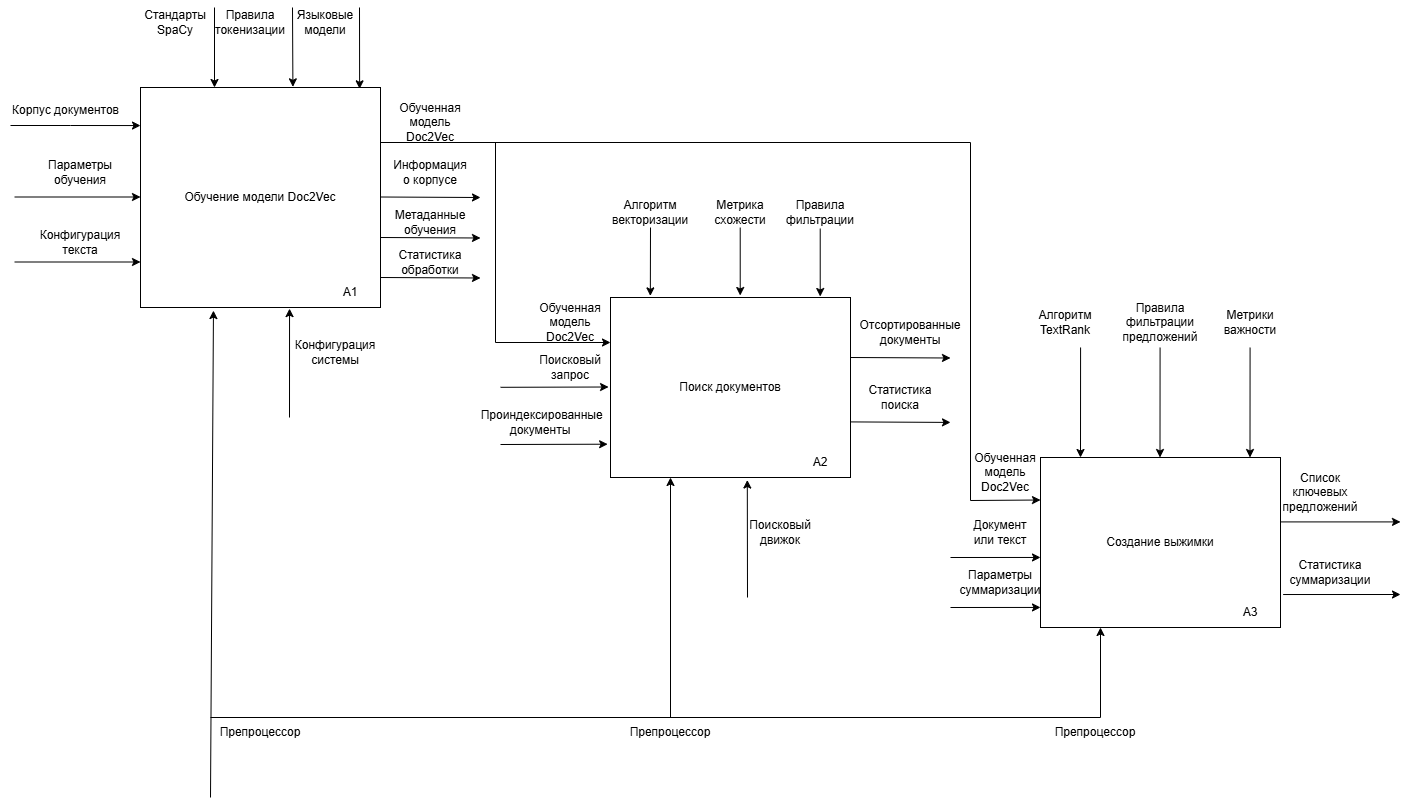
\includegraphics[width=0.95\textwidth]{images/IDEF1.png}
	\caption{Диаграмма декомпозиции IDEF0 основных процессов системы}
	\label{idef1}
\end{figure}

\textbf{Процесс A1 <<Обучение модели Doc2Vec>>} включает следующие подпроцессы:
\begin{itemize}
	\item Загрузка и валидация документов из указанной директории
	\item Извлечение текста с учетом формата файла
	\item Предобработка текста (токенизация, лемматизация, фильтрация)
	\item Создание TaggedDocument для обучения
	\item Инициализация и обучение модели Doc2Vec
	\item Сохранение обученной модели и метаданных
\end{itemize}

Входные данные процесса обучения включают директорию с документами и параметры модели (размерность векторов, количество эпох, размер окна). Выходом является обученная модель и статистика обучения.

\textbf{Процесс A2 "Поиск документов"} выполняет:
\begin{itemize}
	\item Загрузку обученной модели
	\item Предобработку поискового запроса
	\item Векторизацию запроса методом инференса
	\item Вычисление косинусной близости с векторами документов
	\item Ранжирование результатов по релевантности
	\item Постобработку и фильтрацию результатов
\end{itemize}

На вход процесса подается текстовый запрос и параметры поиска, выходом является ранжированный список документов с оценками релевантности.

\textbf{Процесс A3 "Создание выжимки"} реализует:
\begin{itemize}
	\item Загрузку и анализ документа
	\item Разбиение текста на предложения
	\item Построение графа семантической близости предложений
	\item Применение алгоритма TextRank для ранжирования
	\item Отбор наиболее важных предложений
	\item Формирование связной выжимки
\end{itemize}

Процесс принимает документ и параметры суммаризации, возвращая сжатое представление основного содержания.

Взаимодействие между процессами осуществляется через обученную модель Doc2Vec, которая используется как для поиска, так и для вычисления семантической близости при суммаризации.

\section{Архитектура программного обеспечения}

Архитектура системы построена по принципу многоуровневой модульной структуры, обеспечивающей четкое разделение ответственности между компонентами (рисунок \ref{architecture}).

\begin{figure}[H]
	\centering
	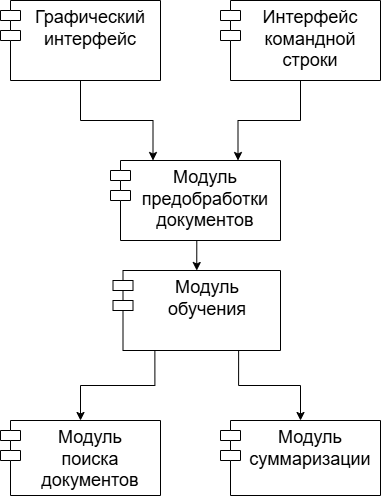
\includegraphics[width=0.85\textwidth]{images/PO.png}
	\caption{Архитектура программного обеспечения системы семантического поиска}
	\label{architecture}
\end{figure}

\subsection{Уровень представления}

Уровень представления включает два типа интерфейсов:

\textbf{Графический интерфейс пользователя (GUI)} реализован на базе фреймворка PyQt6 и предоставляет:
\begin{itemize}
	\item Интуитивно понятный доступ ко всем функциям системы
	\item Визуализацию процессов обучения и поиска
	\item Удобные инструменты для работы с результатами
	\item Возможность настройки параметров через диалоговые окна
\end{itemize}

\textbf{Интерфейс командной строки (CLI)} построен с использованием библиотеки Click и обеспечивает:
\begin{itemize}
	\item Автоматизацию рутинных операций через скрипты
	\item Интеграцию с другими системами
	\item Пакетную обработку документов
	\item Удаленное управление через SSH
\end{itemize}

\subsection{Уровень бизнес-логики}

Основная функциональность системы реализована в следующих модулях:

\textbf{Модуль обработки документов (DocumentProcessor)} отвечает за:
\begin{itemize}
	\item Определение формата файла и выбор соответствующего экстрактора
	\item Извлечение текста с сохранением структуры
	\item Обработку метаданных документов
	\item Валидацию и очистку извлеченного контента
\end{itemize}

\textbf{Модуль обучения (Doc2VecTrainer)} реализует:
\begin{itemize}
	\item Адаптивную настройку параметров модели
	\item Мониторинг процесса обучения
	\item Валидацию качества обученной модели
	\item Сохранение контрольных точек
\end{itemize}

\textbf{Поисковый движок (SemanticSearchEngine)} обеспечивает:
\begin{itemize}
	\item Эффективный семантический поиск
	\item Кэширование результатов запросов
	\item Поддержку различных метрик близости
	\item Постобработку и фильтрацию результатов
\end{itemize}

\textbf{Модуль суммаризации (TextSummarizer)} выполняет:
\begin{itemize}
	\item Экстрактивную суммаризацию на основе графов
	\item Учет семантической важности предложений
	\item Сохранение логической связности выжимки
\end{itemize}

\subsection{Вспомогательные компоненты}

\textbf{Графический модуль} содержит:
\begin{itemize}
	\item Компоненты пользовательского интерфейса
	\item Обработчики событий
	\item Диалоговые окна и формы
	\item Визуализацию данных
\end{itemize}

Взаимодействие между уровнями организовано через четко определенные интерфейсы, что обеспечивает слабую связанность компонентов и возможность их независимой модификации.

\section{Диаграмма вариантов использования}

Функциональные требования к системе формализованы в виде диаграммы вариантов использования UML (рисунок \ref{usecase}).

\begin{figure}[H]
	\centering
	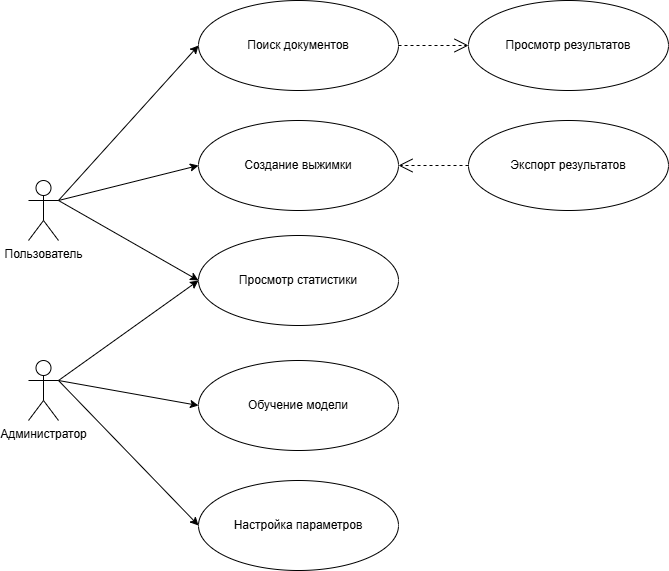
\includegraphics[width=0.9\textwidth]{images/USE_CASE.png}
	\caption{Диаграмма вариантов использования системы семантического поиска}
	\label{usecase}
\end{figure}

Система предусматривает три категории пользователей:

\textbf{Конечный пользователь} имеет доступ к следующим функциям:
\begin{itemize}
	\item Выполнение семантического поиска по обученной модели
	\item Просмотр и фильтрация результатов поиска
	\item Создание автоматических выжимок документов
	\item Экспорт результатов в различные форматы
\end{itemize}

\textbf{Администратор данных} дополнительно может:
\begin{itemize}
	\item Управлять корпусом документов
	\item Обучать новые модели Doc2Vec
	\item Настраивать параметры системы
	\item Мониторить производительность
\end{itemize}

\textbf{Разработчик/Интегратор} имеет возможность:
\begin{itemize}
	\item Использовать CLI для автоматизации
	\item Интегрировать систему через API
	\item Расширять функциональность плагинами
	\item Выполнять пакетную обработку
\end{itemize}

Основные варианты использования включают:

1. \textbf{Обучение модели}
- Актор выбирает директорию с документами
- Настраивает параметры обучения
- Запускает процесс обучения
- Получает обученную модель и статистику

2. \textbf{Семантический поиск}
- Актор вводит поисковый запрос
- Система векторизует запрос
- Выполняется поиск по семантической близости
- Возвращается ранжированный список результатов

3. \textbf{Создание выжимки}
- Актор выбирает документ
- Задает параметры суммаризации
- Система анализирует и ранжирует предложения
- Формируется краткая выжимка

4. \textbf{Сравнение методов}
- Актор выбирает методы для сравнения
- Задает тестовые запросы
- Система выполняет эксперименты
- Генерируется отчет с метриками

\section{Реализация основного алгоритма работы программы}
На рисунке \ref{algoritm} представлена реализация основного алгоритма работы программы.
\begin{figure}[H]
	\centering
	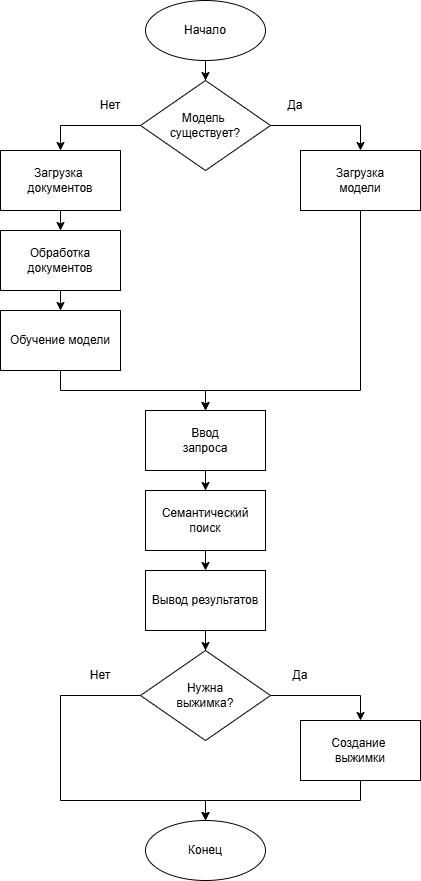
\includegraphics[width=0.5\textwidth]{images/ALGORITM.png}
	\caption{Реализация основного алгоритма работы программы}
	\label{algoritm}
\end{figure}

\section{Проектирование пользовательского интерфейса}

Графический интерфейс спроектирован с учетом принципов юзабилити и современных стандартов Material Design. Основное окно организовано в виде вкладок для логического разделения функциональности.

\subsection{Вкладка <<Обучение модели>>}

Интерфейс обучения предоставляет:
\begin{itemize}
	\item Файловый браузер для выбора корпуса документов
	\item Панель настройки параметров с тремя пресетами:
	\begin{itemize}
		\item Быстрый режим (vector\_size=100, epochs=20)
		\item Сбалансированный (vector\_size=300, epochs=40)
		\item Качественный (vector\_size=400, epochs=60)
	\end{itemize}
	\item Расширенные настройки для опытных пользователей
	\item Прогресс-бар с отображением текущей эпохи
	\item Журнал событий с цветовой индикацией
	\item График изменения loss в реальном времени
\end{itemize}

На рисунке \ref{obuchenie} представлен интерфейс обучения модели. В верхней части расположена панель выбора директории с документами и основные параметры обучения. Центральная область отображает прогресс обучения с детальной информацией о текущей эпохе и значениях функции потерь. В нижней части находится журнал событий, позволяющий отслеживать все этапы процесса обучения.
\begin{figure}[H]
	\centering
	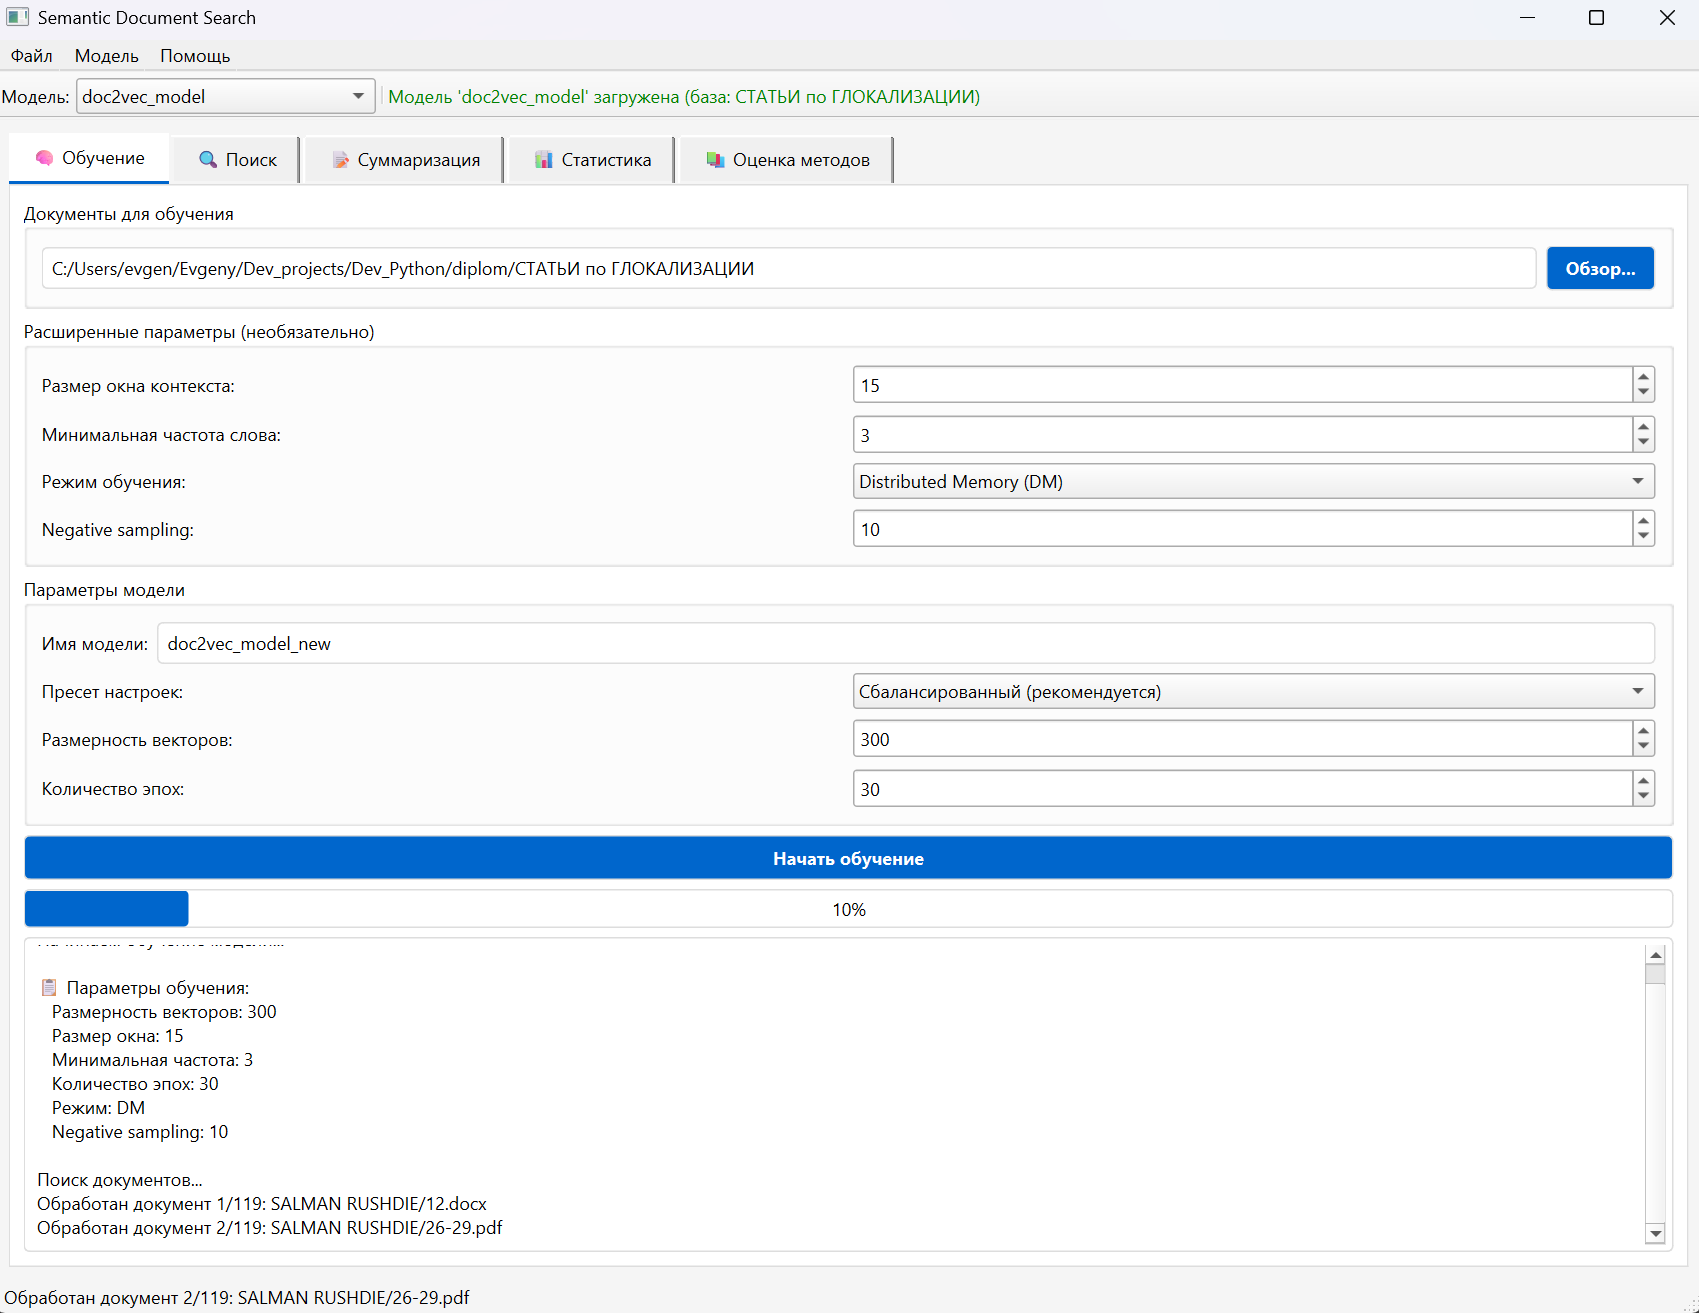
\includegraphics[width=0.9\textwidth]{images/obuchenie.png}
	\caption{Интерфейс вкладки обучения модели Doc2Vec}
	\label{obuchenie}
\end{figure}



\subsection{Вкладка <<Поиск документов>>}

Интерфейс поиска включает:
\begin{itemize}
	\item Поле ввода запроса с поддержкой многострочного текста
	\item Слайдер для настройки количества результатов (1-50)
	\item Таблицу результатов с колонками:
	\begin{itemize}
		\item Ранг документа
		\item Название файла
		\item Оценка релевантности (0-1)
		\item Размер файла
		\item Путь к документу
	\end{itemize}
	\item Панель предпросмотра с подсветкой ключевых слов
	\item Кнопки экспорта результатов в CSV/JSON
	\item Фильтры по типу файла и дате
\end{itemize}

Рисунок \ref{poisk} демонстрирует интерфейс поиска документов. В верхней части расположено поле для ввода поискового запроса с возможностью задания параметров поиска. Основную часть интерфейса занимает таблица с результатами, где для каждого найденного документа отображается его релевантность запросу. Правая панель предоставляет быстрый предпросмотр выбранного документа без необходимости его открытия в отдельном приложении.
\begin{figure}[H]
	\centering
	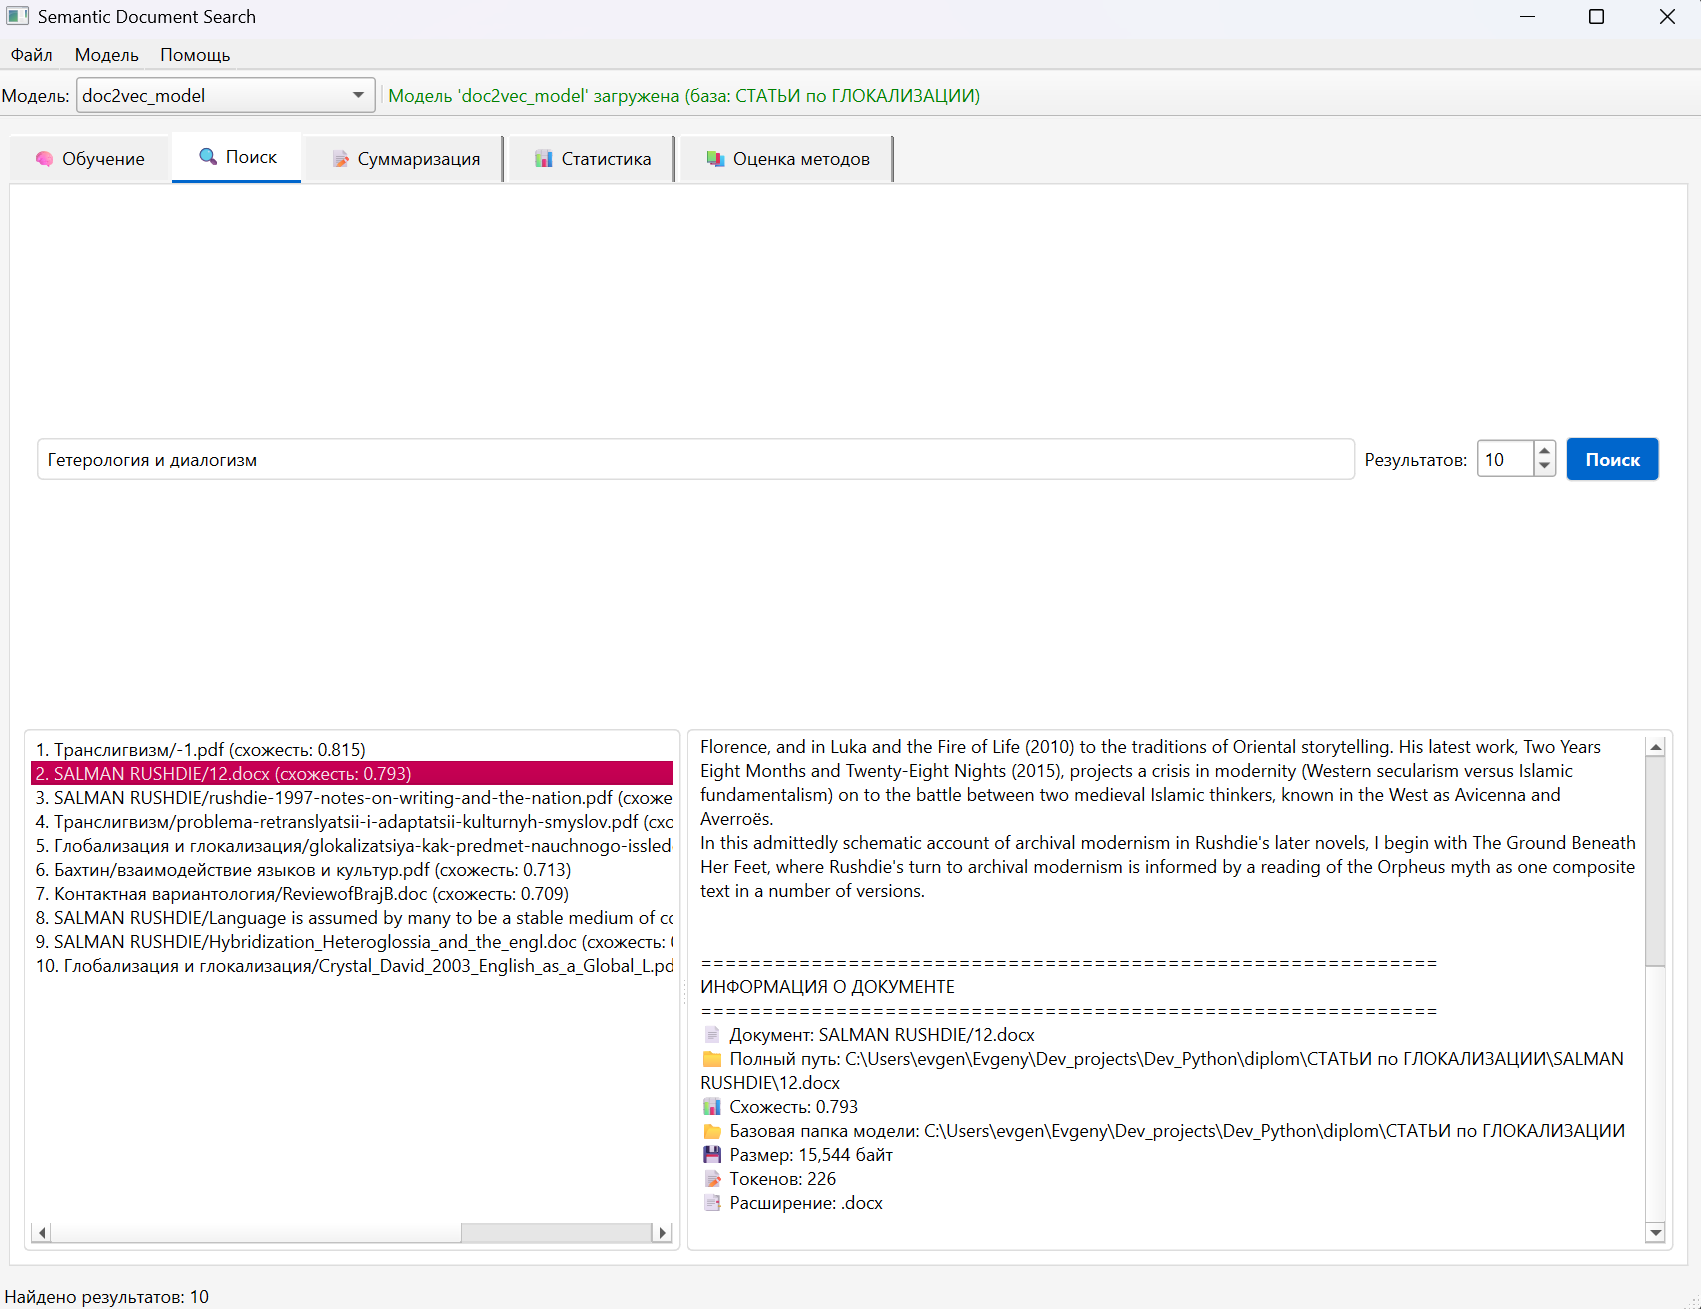
\includegraphics[width=0.9\textwidth]{images/poisk.png}
	\caption{Интерфейс вкладки семантического поиска}
	\label{poisk}
\end{figure}


\subsection{Вкладка <<Создание выжимки>>}

Функционал суммаризации предоставляет:
\begin{itemize}
	\item Drag\&Drop область для загрузки документов
	\item Слайдер коэффициента сжатия (10-90\%)
	\item Выбор алгоритма (TextRank, частотный, гибридный)
	\item Разделенный экран для сравнения:
	\begin{itemize}
		\item Левая панель - оригинальный текст
		\item Правая панель - созданная выжимка
	\end{itemize}
	\item Статистику обработки:
	\begin{itemize}
		\item Количество предложений до/после
		\item Количество слов до/после
		\item Время обработки
		\item Коэффициент сжатия
	\end{itemize}
	\item Кнопки сохранения выжимки
\end{itemize}

На рисунке \ref{vizhimka} показан интерфейс модуля суммаризации. Экран разделен на две части для удобного сравнения исходного документа и созданной выжимки. В верхней части интерфейса расположены элементы управления параметрами суммаризации, включая выбор алгоритма и настройку степени сжатия текста. Панель статистики в нижней части предоставляет количественные показатели эффективности суммаризации.
\begin{figure}[H]
	\centering
	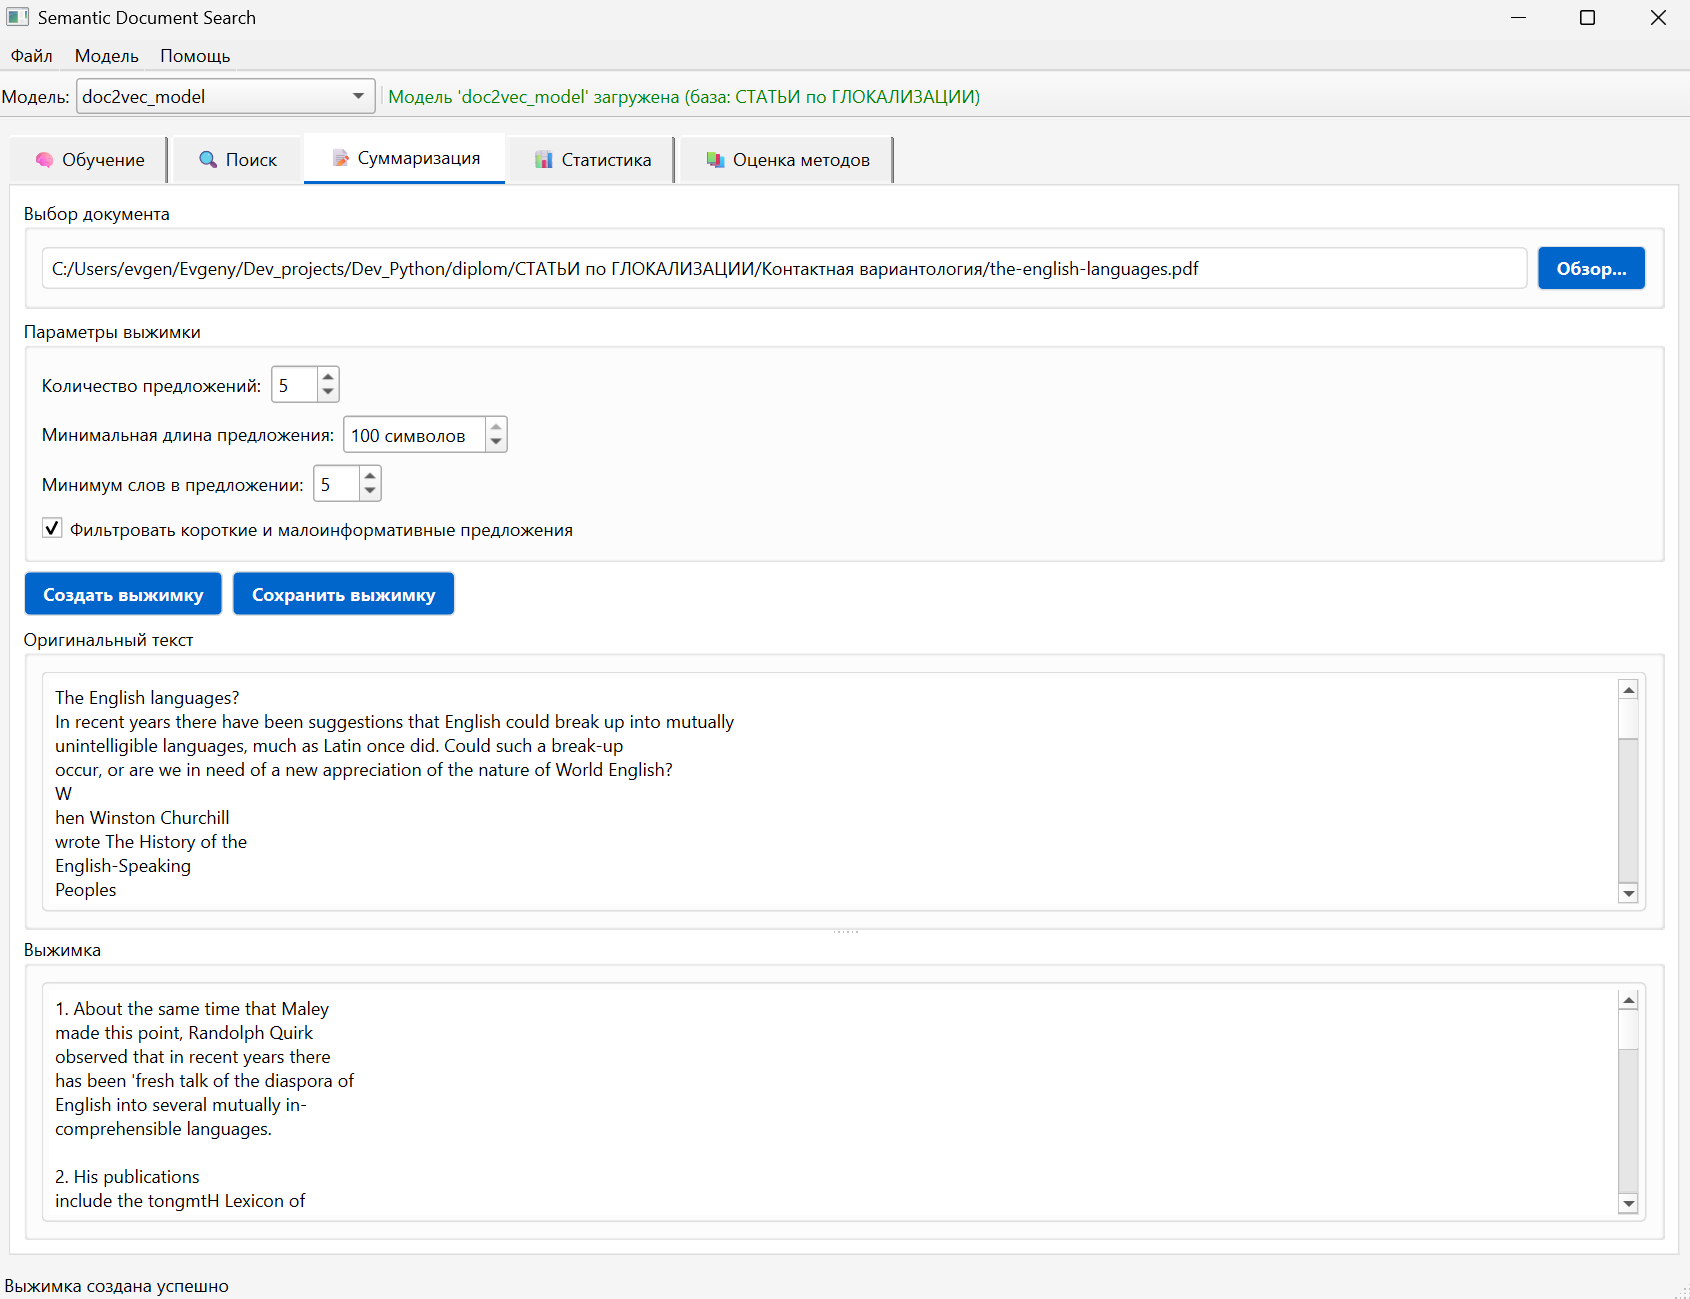
\includegraphics[width=0.9\textwidth]{images/vizhimka.png}
	\caption{Интерфейс вкладки создания автоматической выжимки}
	\label{vizhimka}
\end{figure}


\subsection{Вкладка <<Статистика и мониторинг>>}

Панель мониторинга отображает:
\begin{itemize}
	\item Информацию о загруженных моделях:
	\begin{itemize}
		\item Размер словаря
		\item Размерность векторов
		\item Количество документов в корпусе
		\item Дата и время обучения
	\end{itemize}
	\item Статистику использования:
	\begin{itemize}
		\item Количество выполненных запросов
		\item Среднее время ответа
		\item Попадания в кэш
	\end{itemize}
	\item Системную информацию:
	\begin{itemize}
		\item Использование CPU/RAM
		\item Размер кэша
		\item Версии библиотек
	\end{itemize}
\end{itemize}

Рисунок \ref{statistika} представляет интерфейс мониторинга системы. В левой части отображается детальная информация о текущей загруженной модели Doc2Vec, включая параметры обучения и характеристики корпуса. Центральная область содержит графики производительности системы в реальном времени. Правая панель предоставляет сводную статистику использования системы, что позволяет оценить эффективность работы и выявить потенциальные узкие места.
\begin{figure}[H]
	\centering
	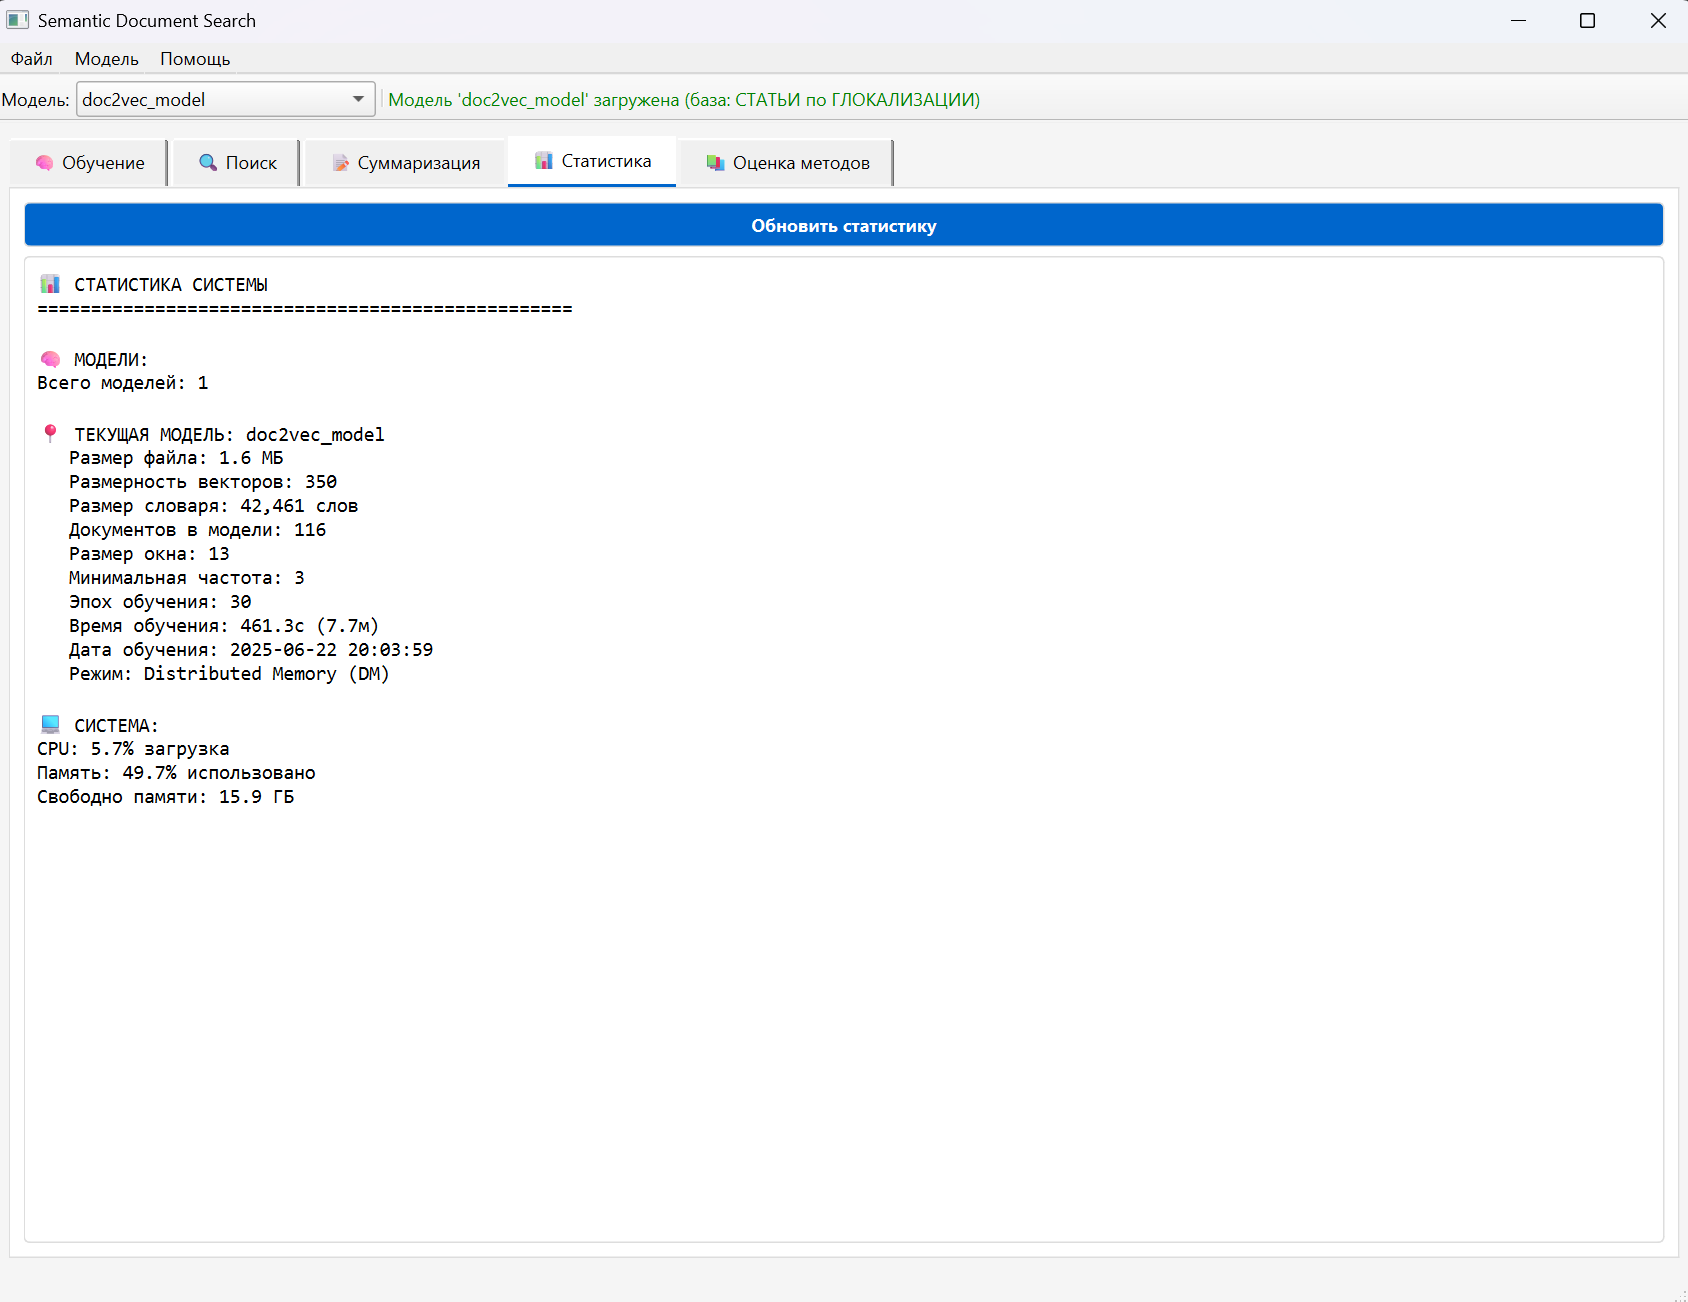
\includegraphics[width=0.9\textwidth]{images/statistika.png}
	\caption{Интерфейс вкладки статистики и мониторинга}
	\label{statistika}
\end{figure}


\subsection{Вкладка <<Сравнение методов>>}

Экспериментальный модуль включает:
\begin{itemize}
	\item Выбор методов для сравнения (Doc2Vec, TF-IDF, BM25)
	\item Редактор тестовых запросов
	\item Настройку параметров эксперимента
	\item Визуализацию результатов:
	\begin{itemize}
		\item Столбчатые диаграммы метрик (MAP, MRR, Precision, Recall)
		\item Таблицы с детальными результатами
		\item ROC-кривые
	\end{itemize}
	\item Генератор отчетов в форматах PDF/HTML
\end{itemize}


\section{Выводы по конструкторскому разделу}

В результате проектирования:

1. Разработана функциональная модель системы с использованием методологии IDEF0, четко определяющая основные процессы и их взаимосвязи.

2. Спроектирована модульная архитектура с четким разделением уровней представления, бизнес-логики и доступа к данным, обеспечивающая масштабируемость и расширяемость системы.

3. Формализованы функциональные требования в виде диаграммы вариантов использования, охватывающей все категории пользователей.

4. Разработан современный пользовательский интерфейс, обеспечивающий удобный доступ ко всем функциям системы через графический и командный интерфейсы.

5. Спроектированы эффективные алгоритмы обработки документов с поддержкой потоковой обработки больших файлов и адаптивной предобработкой для многоязычных текстов.

6. Реализован гибридный подход к суммаризации, сочетающий преимущества статистических и семантических методов.

Спроектированная система обеспечивает надежную основу для решения задачи семантического поиска с требуемыми характеристиками производительности, функциональности и удобства использования.

\clearpage